\section{Introduction}

This chapter documents the practical implementation of the Mosaned system. It presents the realized management dashboard, the mobile application, the obstacle detection hardware, and the process of QR code integration in indoor spaces. Screenshots and photographs provide evidence of the working system and support the overall workflow described in the previous chapters.

\section{Management Dashboard}

As mentioned in the methodology chapter, the management dashboard enables administrators to control building navigation data. The implemented system includes a secure login screen, shown in \autoref{fig:dashboard-login}, which restricts access to authorized users only.
\begin{figure}[h]
	\centering
	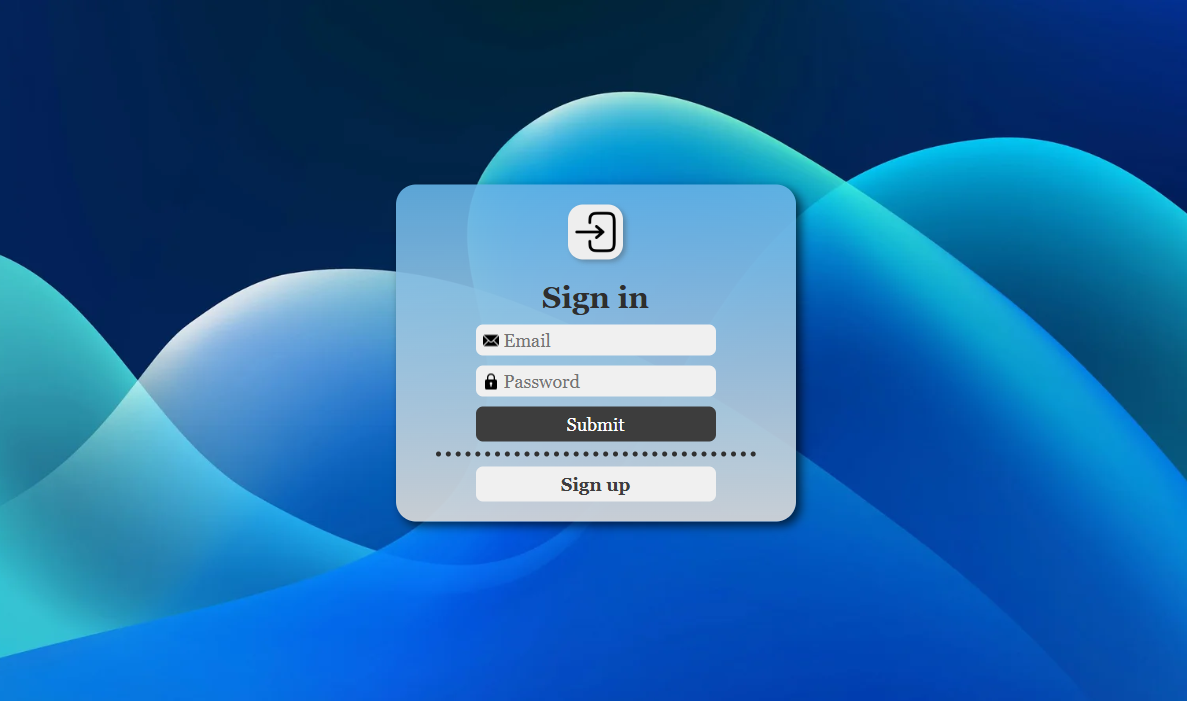
\includegraphics[width=1\textwidth]{assets/ch5_imp/login_page.png}
	\caption{Login screen of the Mosaned management dashboard, ensuring secure access for authorized administrators.}
	\label{fig:dashboard-login}
\end{figure}

After authentication, administrators access the main dashboard interface (\autoref{fig:dashboard-main}), which displays managed buildings and provides options for adding or editing records. This interface was implemented to facilitate streamlined navigation and quick data management.
\begin{figure}[h]
	\centering
	\includegraphics[width=0.8\textwidth]{example-image-b}
	\caption{Main dashboard interface showing the list of managed buildings, with options for adding new buildings or editing existing ones.}
	\label{fig:dashboard-main}
\end{figure}

QR code generation and assignment are performed through a dedicated management page (\autoref{fig:dashboard-qr-management}). This page allows batch operations and contextual instruction editing, as required for scalable deployments.
\begin{figure}[h]
	\centering
	\includegraphics[width=0.8\textwidth]{example-image-c}
	\caption{QR code management page, enabling administrators to generate, edit, and assign instructions to QR codes for specific locations within a building.}
	\label{fig:dashboard-qr-management}
\end{figure}

\section{Mobile Application}

The mobile application, as detailed in the methodology chapter, was implemented to provide users with seamless access to indoor navigation and real-time guidance. The home screen (\autoref{fig:app-home}) was designed to deliver immediate access to key functions, based on user feedback during early prototyping.
\begin{figure}[h]
	\centering
	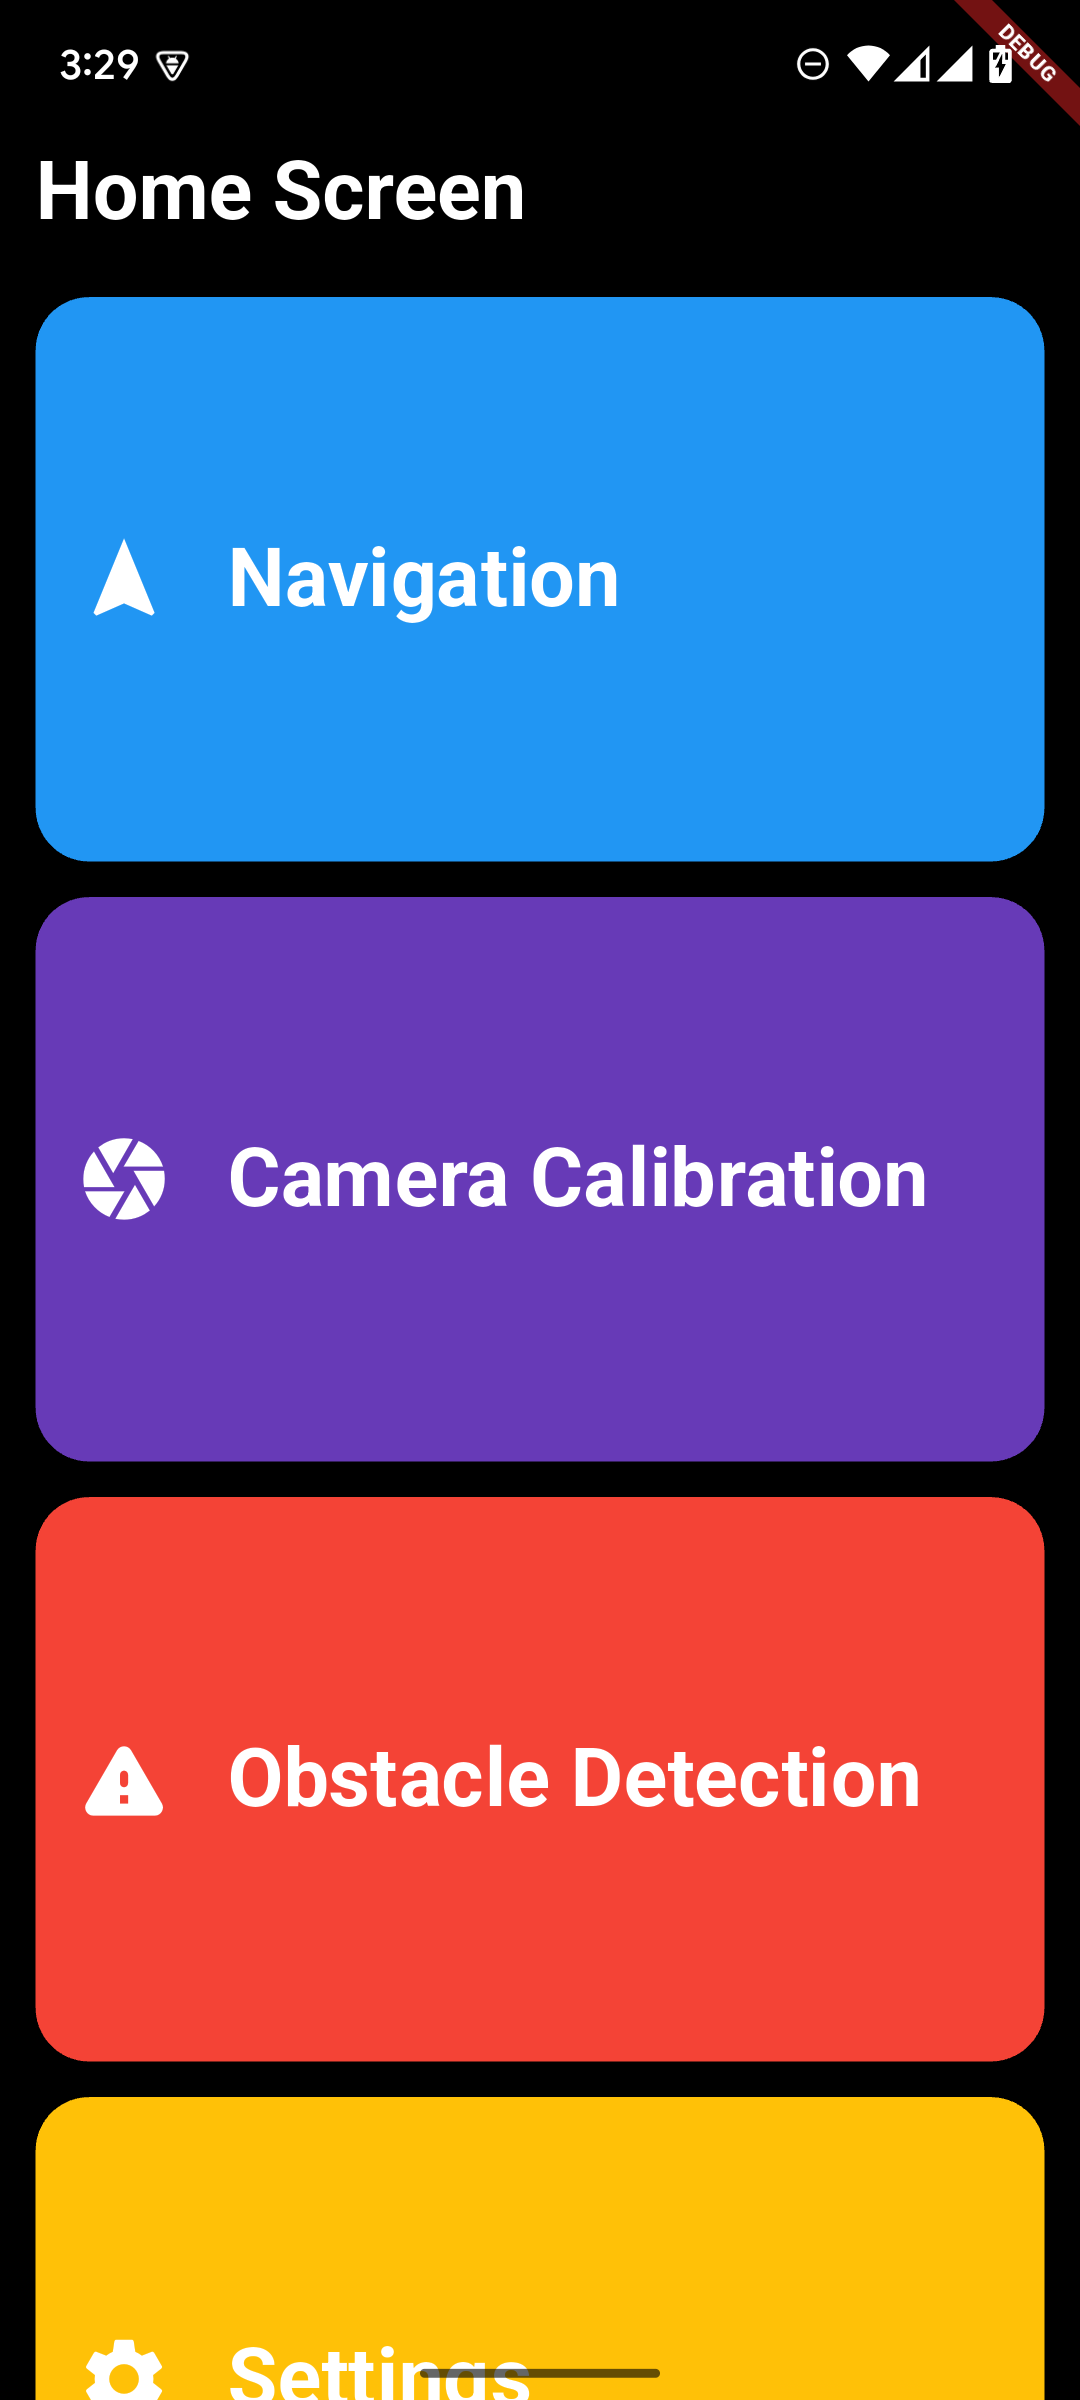
\includegraphics[width=0.5\textwidth]{assets/ch5_imp/mobile_app_homescreen.png}
	\caption{Home screen of the Mosaned mobile application, providing quick access to navigation and settings.}
	\label{fig:app-home}
\end{figure}

A dedicated interface for QR code scanning was developed, as shown in \autoref{fig:app-qr-scan}, enabling accurate user localization and retrieval of contextual navigation instructions.
\begin{figure}[h]
	\centering
	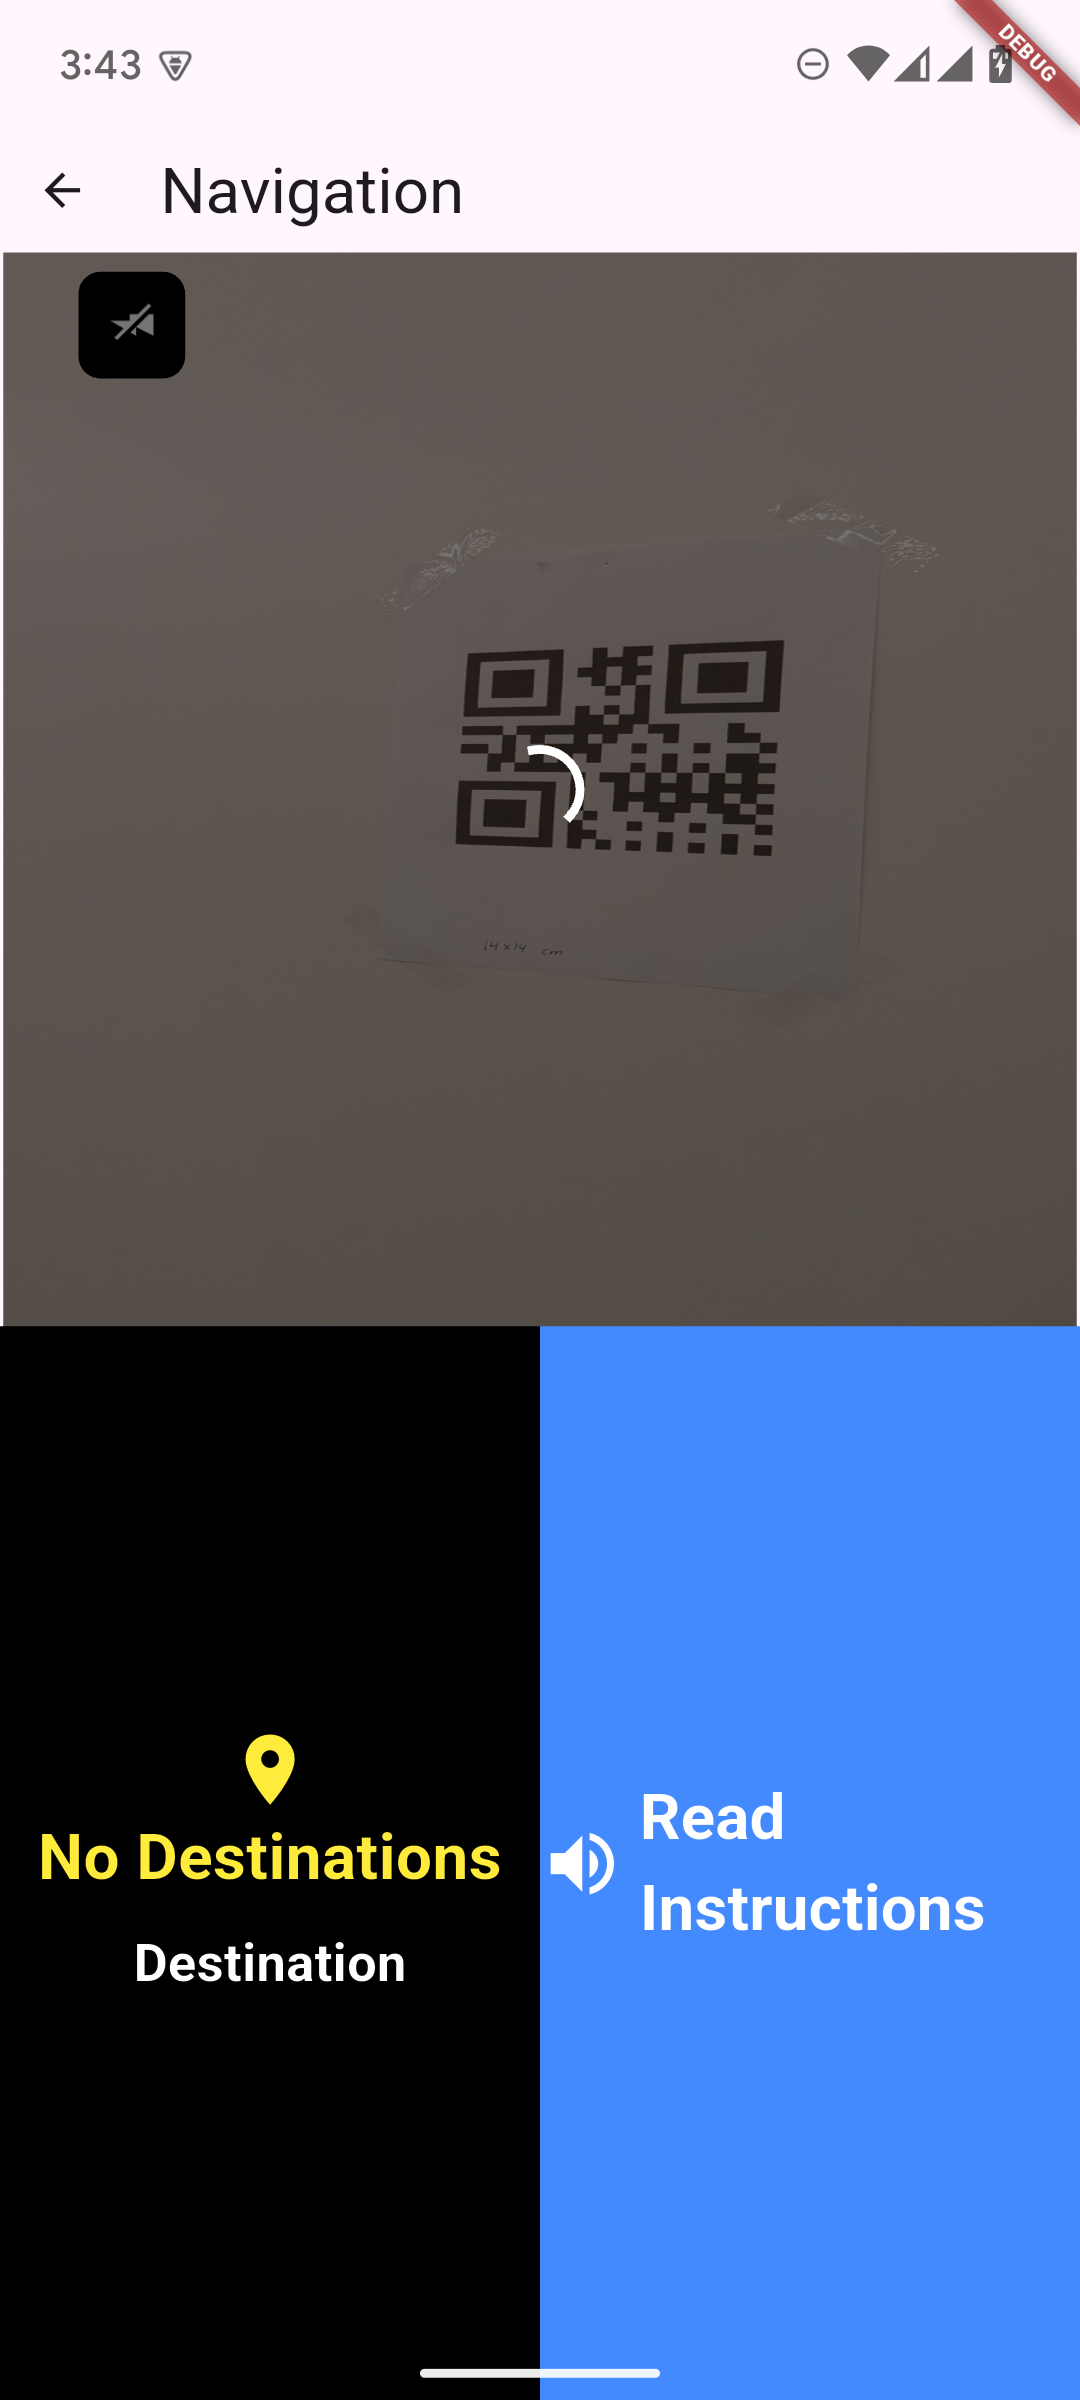
\includegraphics[width=0.5\textwidth]{assets/ch5_imp/mobile_app_navscreen.png}
	\caption{QR code scanning interface, allowing the user to localize themselves within the building and retrieve contextual instructions.}
	\label{fig:app-qr-scan}
\end{figure}

\section{Obstacle Detection Hardware}

The implementation of the obstacle detection hardware followed the approach outlined in the methodology chapter. The assembled module, shown in \autoref{fig:hardware-overview}, combines the microcontroller and sensor elements on a compact board.
\begin{figure}[h]
	\centering
	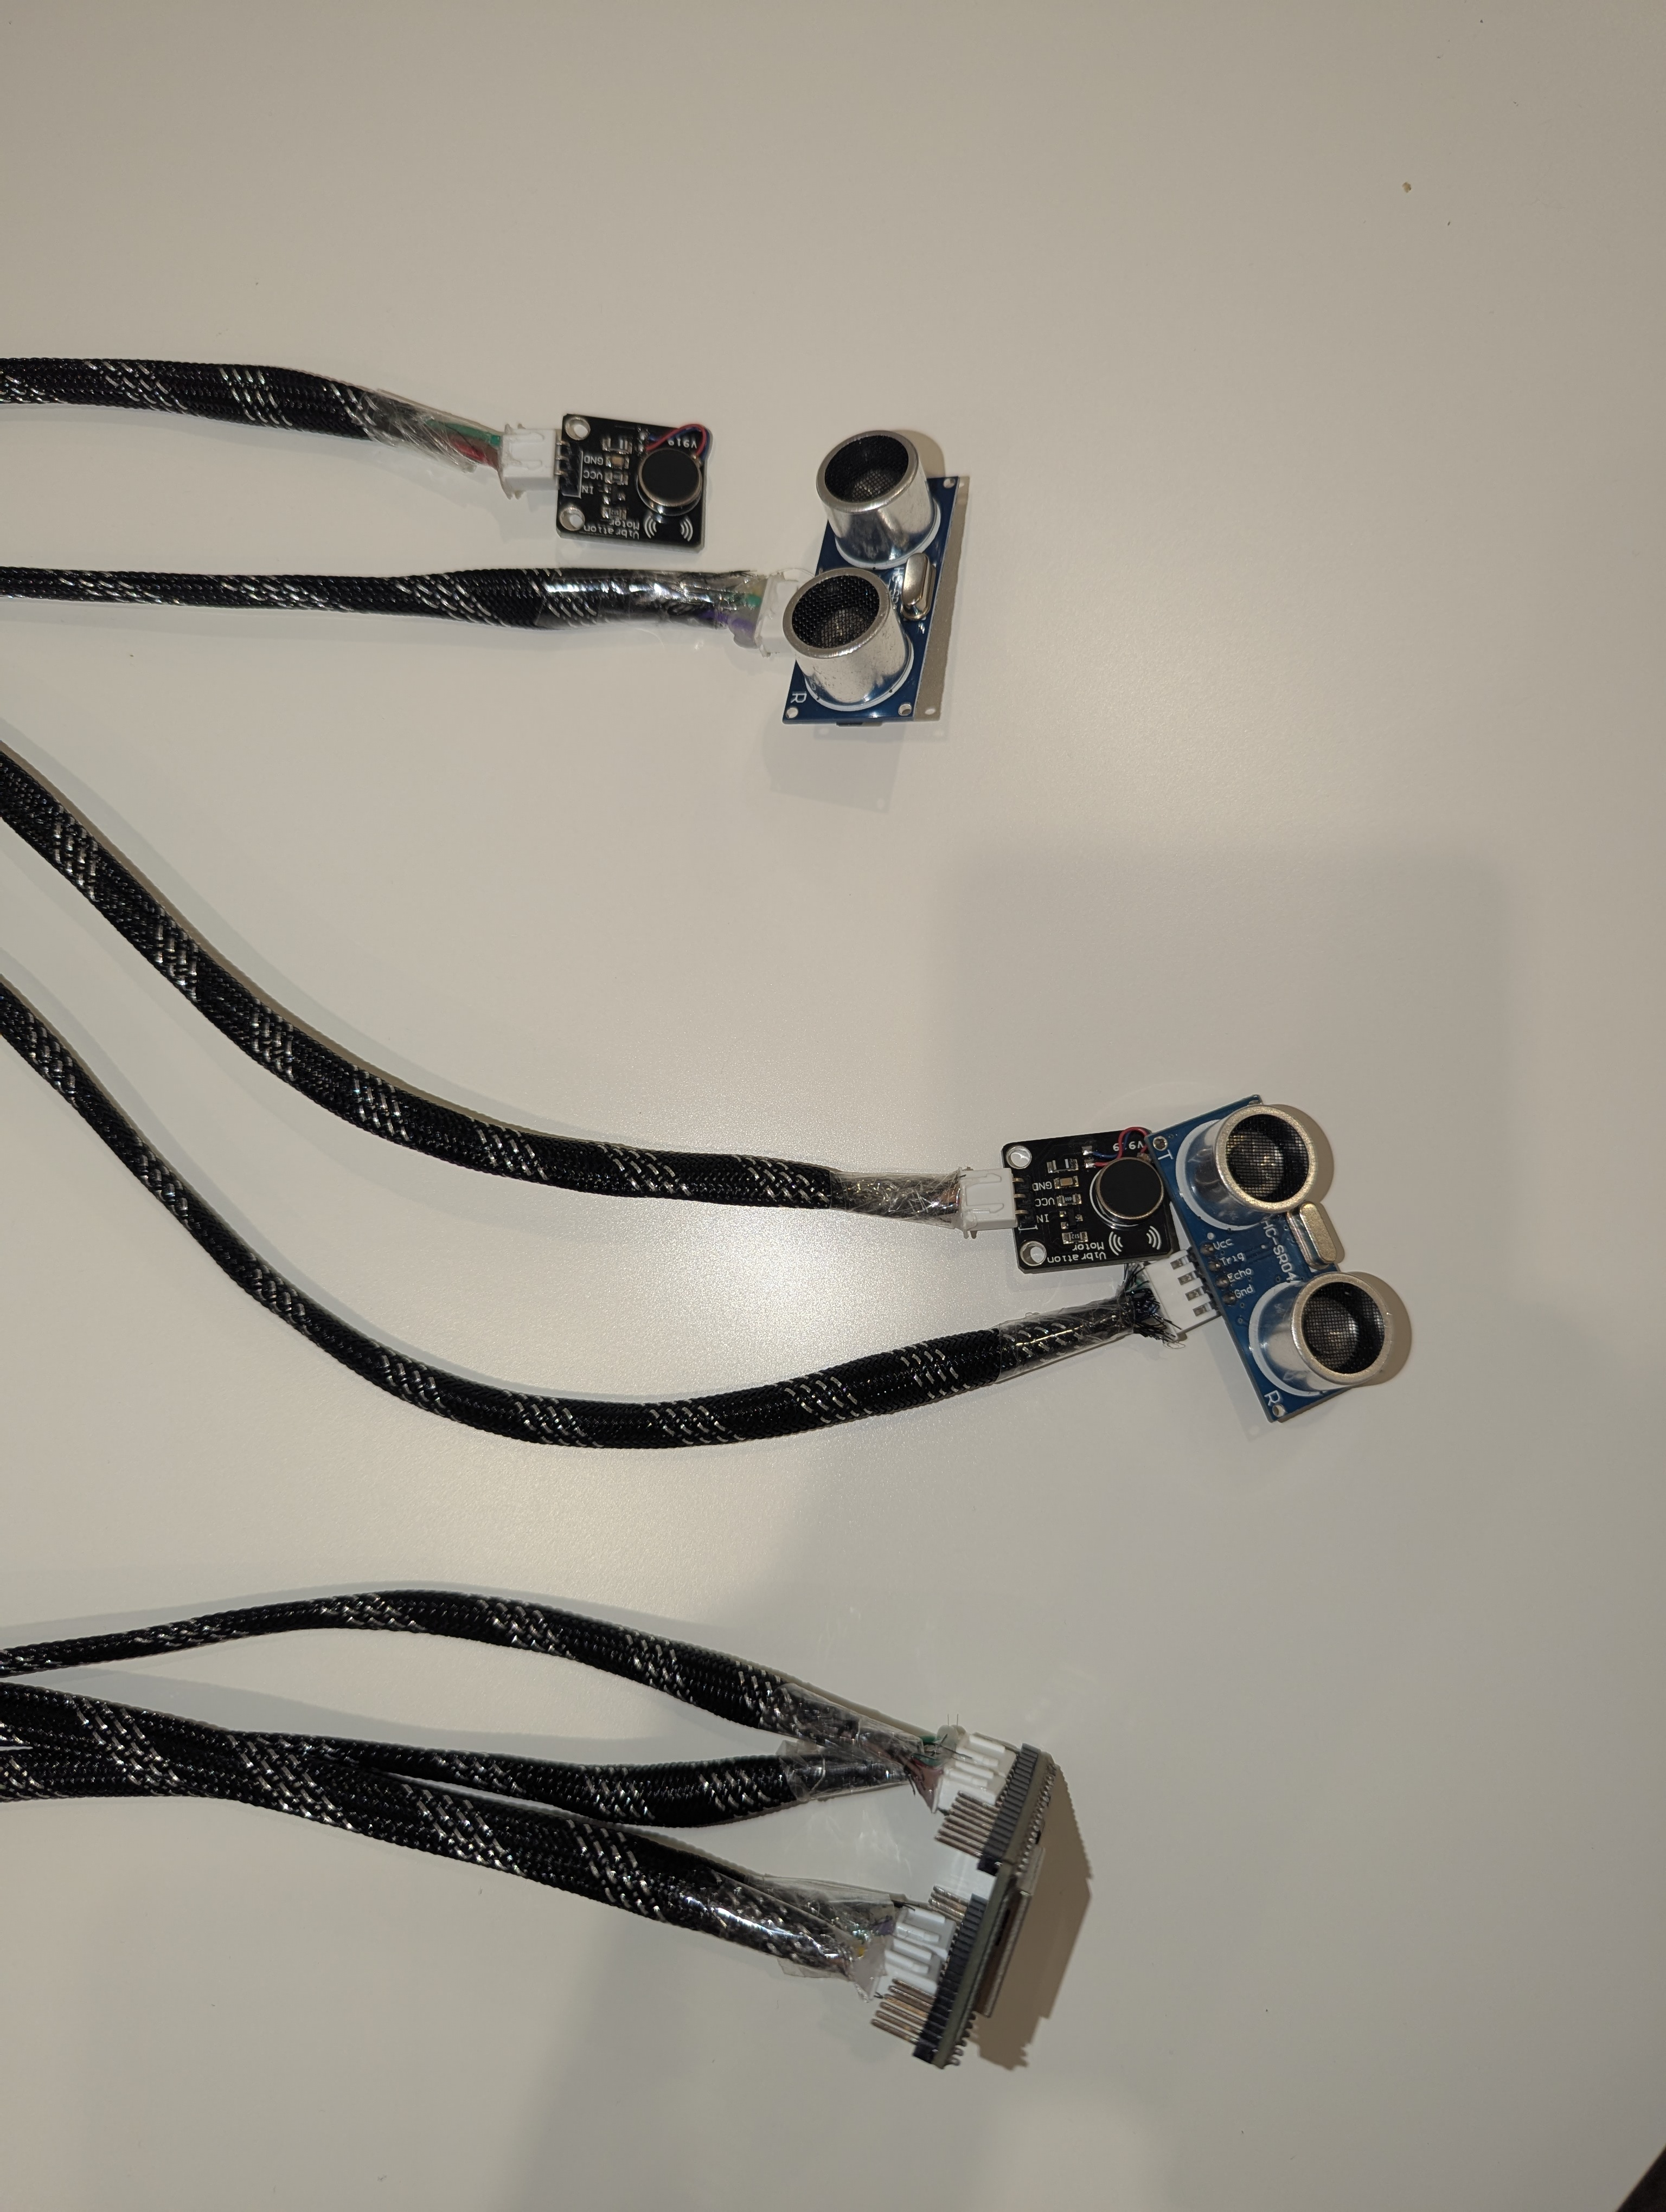
\includegraphics[width=0.7\textwidth]{assets/ch5_imp/obstacle_detection.jpg}
	\caption{Assembled obstacle detection module showing the ESP32 board, connected ultrasonic sensors, and coin vibration motors.}
	\label{fig:hardware-overview}
\end{figure}

The final wearable setup was tested for comfort and ease of use, as illustrated in \autoref{fig:hardware-wearable}. The modular design allowed rapid iteration based on user feedback.
\begin{figure}[h]
	\centering
	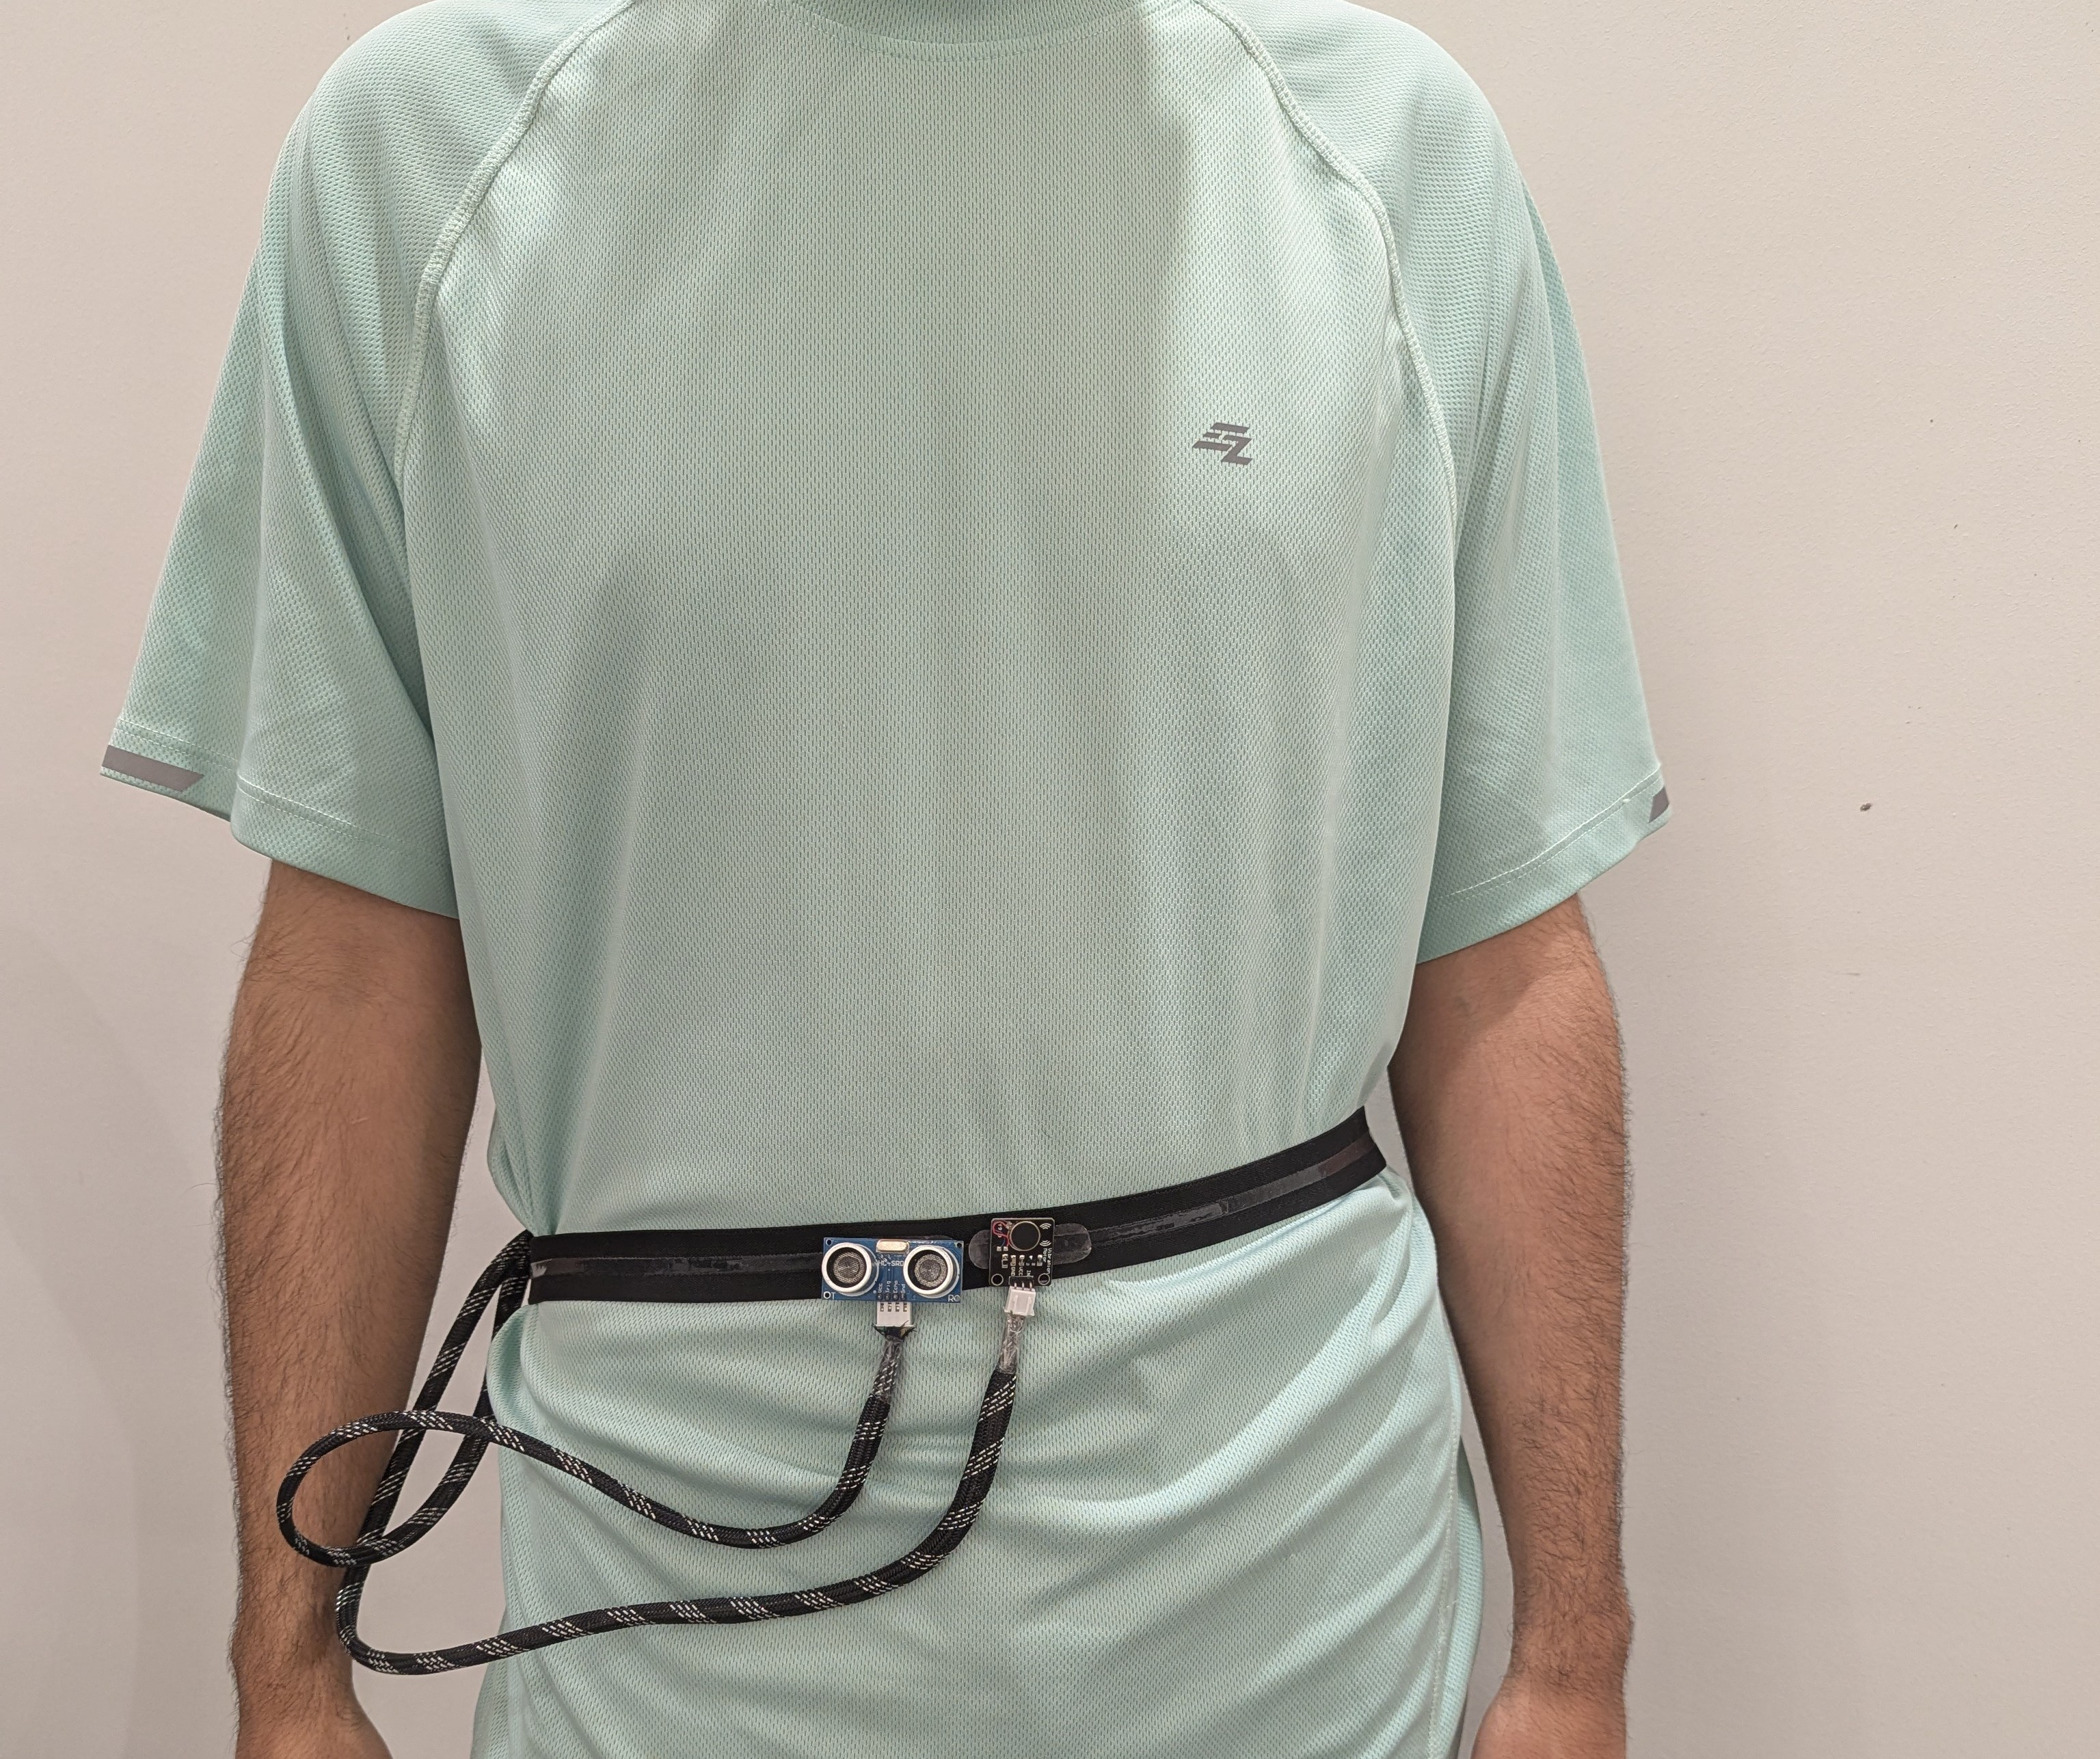
\includegraphics[width=0.7\textwidth]{assets/ch5_imp/obstac_weared.jpg}
	\caption{Wearable setup of the obstacle detection system, designed for user comfort and mobility.}
	\label{fig:hardware-wearable}
\end{figure}

\bigskip

This chapter demonstrates the practical realization of Mosaned, with each figure providing visual documentation for the developed components and the overall implementation approach.
